\chapter{Pian cu Arduino}
\section {Descrierea componentelor}
\myindent

\vspace{5mm}
Schema circuitului cuprinde: 
\begin{enumerate}
\color{ForestGreen}
\item 11 butoane
\item 11 LED-uri
\item 11 rezistoare de 5$K\Omega$
\item 1 rezistor de 220$\Omega$
\item 1 difuzor
\item 2 t'abli'te Breadboard
\item 1 placa Arduino Uno R3
\item 53 de fire de dimensiuni diferite
\end{enumerate}

\vspace{5mm}
\myindent
\textbf {Arduino Uno} este un microcontroller provenit de la microcontroller-ul ATmega328P. Acesta are 14 intr'ari/ie'siri digitale sub form'a de pini (din care 6 pot fi folosite ca ie'siri PWM), 6 intr'ari analogice, un rezonator ceramic de 16 MHz (CSTCE16M0V53-R0), un port USB, un port jack de alimentare, un port ICSP 'si un buton de resetare.

Aceast'a pl'acu'ta vine la pachet si cu un program software cu un limbaj asemanator cu C/C++ prin care se poate manipula cu u'surin't'a functionarea microcontroller-ului. De asemenea, exist'a 'si o variant'a cu limbaj Blocky care este cel mai usor 'si mai intuitiv limbaj de programare pentru pl'acu'tele Arduino.

\section{Descrierea circuitului}
\myindent
Acest circuit folose'ste Pl'acu'ta Arduino pentru a scoate sunetele unui pian folosind un difuzor. Pl'acu'ta a fost programat'a s'a scoat'a prin difuzor anumite frecven'te care sunt percepute de oameni ca ni'ste sunete cu intensit'a'ti diferite. Aceste frecven'te sunt eliberate 'in momentul 'in care se apas'a butoanele circuitului. Pentru acest circuit butonul cel mai din st\^anga scoate frecven'ta cea mai mic'a, iar butonul cel mai din dreapta scoate frecven'ta cea mai mare. Cre'sterea frecven'telor se face progresiv de la st\^anga la dreapta. 'In cazul 'in care se apas'a mai multe butoane deodat'a se va "alege" butonul cu frecven'ta cea mai mic'a, deoarece programul din microcontroller verific'a butoanele de la st\^anga la dreapta.\\

\vspace{5mm}
Programul folosit pentru setarea pl'acu'tei Arduino este:
\begin{verbatim}
//Declararea de variabile
int button1 = 2;	// Asocierea butoanelor cu numerele de pe
int button2 = 3;	// placuta Arduino.
int button3 = 4;
int button4 = 5;
int button5 = 6;
int button6 = 7;
int button7 = 8;
int button8 = 9;
int button9 = 10;
int button10 = 11;
int button11 = 12;

int piezo = 13;		// Asocierea difuzorului

int a, b, c, d, e, f, g, h, i, j, k; // Asocierea variabilelor pentru output

// Configurarea placii Arduino
void setup()
{
// Initializarea comunicarii
  Serial.begin(9600);		
  
// Configurarea pinilor pentru receptionarea semnalului cu ajutorul butoanelor
  pinMode(button1,INPUT);	
  pinMode(button2,INPUT); 
  pinMode(button3,INPUT);
  pinMode(button4,INPUT);
  pinMode(button5,INPUT);
  pinMode(button6,INPUT);
  pinMode(button7,INPUT);
  pinMode(button8,INPUT);
  pinMode(button9,INPUT);
  pinMode(button10,INPUT);
  pinMode(button11,INPUT);
}

// Programarea placii Arduino
void loop()
{
// Citirea datelor de intrare prin variabilele de output
  a = digitalRead(button1);	
  b = digitalRead(button2);
  c = digitalRead(button3);
  d = digitalRead(button4);
  e = digitalRead(button5);
  f = digitalRead(button6);
  g = digitalRead(button7);
  h = digitalRead(button8);
  i = digitalRead(button9);
  j = digitalRead(button10);
  k = digitalRead(button11);
 
// si trimiterea rezultatului catre Piezo a unei frecvente de vibrare
// astfel incat sa scoata sunete cat mai intense cu apasarea
// butoanelor de la stanga la dreapta sau nici un sunet daca nu e apasat
// nici un buton
  if(a == 1){				
    tone(piezo,523);	
  } else if(b == 1){
    tone(piezo,575);		
  } else if(c == 1){			
    tone(piezo,628);
  } else if(d == 1){
    tone(piezo,681);
  } else if(e == 1){
    tone(piezo,733);
  } else if(f == 1){
    tone(piezo,786);
  } else if(g == 1){
    tone(piezo,838);
  } else if(h == 1){
    tone(piezo,890);
  } else if(i == 1){
    tone(piezo,943);
  } else if(j == 1){
    tone(piezo,995);
  } else if(k == 1){
    tone(piezo,1047);
  } else{
    noTone(piezo);
  }  
  delay(50);}
\end{verbatim}

\section{Link-uri 'si scheme}
\myindent
Link-ul circuitului: \url{https://www.tinkercad.com/things/dIhJH05zwqa-arduino-circuit}

\vspace{10mm}
\begin{figure}[ht]
\centering
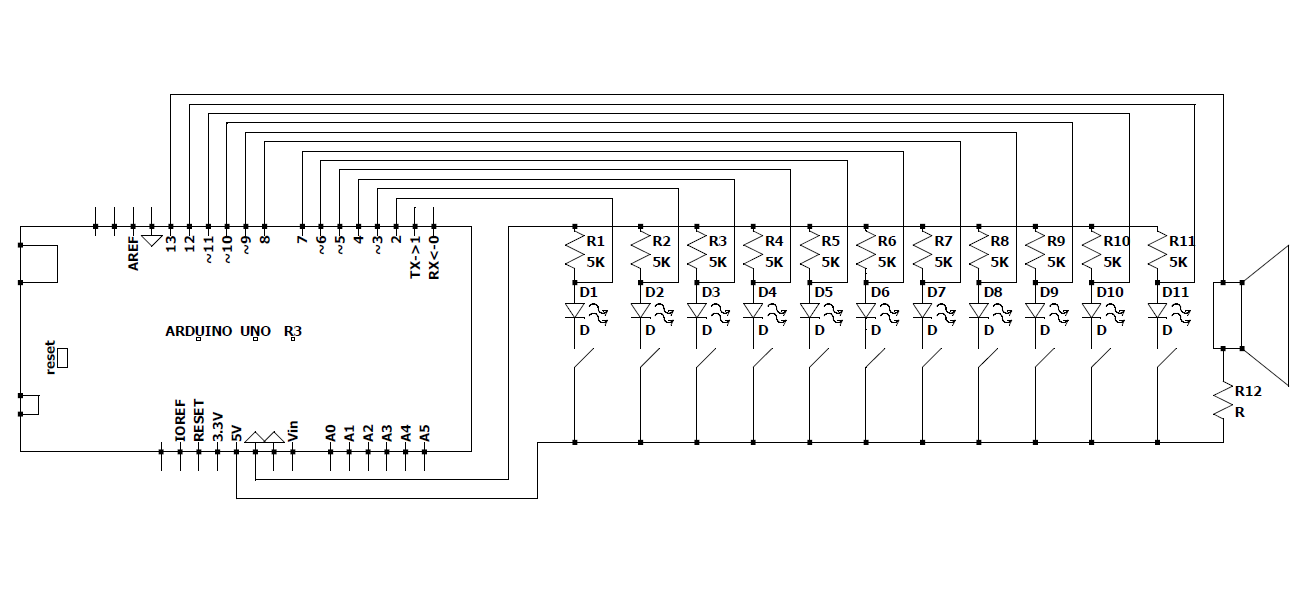
\includegraphics[scale=0.5]{Fisiere/Schema Arduino}
\caption {Schema circuitului implementat'a in LTSpice}
\end{figure}
\FloatBarrier